\chapter{Introduction}
\label{ch:intro}
%
As science and technology evolves, a myriad of data collections are produced. The common denominator of all these data collections is the same -- they are regarded as containing useful and usable information from which actionable evidence can be extracted, the latter leading to improvements in many directions -- increased sales, better customer support, more accurate assessments of phenomena, or, at a higher level, the advance of understanding of these phenomena that have created the data, and, thereby, an increase of knowledge and advancement to science. These datasets challenge their consumers in many ways. Several relevant aspects that induce such challenges include the \emph{size} of datasets (the `big data' revolution has made the efficient processing of terrabyte dataset collections a mandatory requirement for most application areas); the \emph{quality} of data (principled statistical analysis and modeling of phenomena captured by data require accurately measured and collected datasets); and the \emph{provenance} of data (one needs to know how the entire end-to-end pipeline of obtaining a given dataset looks like before being able to make strong statements concerning insights derived from the respective data).

Yet, the challenges of understanding data are not limited to the above issues. A separate, and equally important, one regards the \emph{structure} of data itself. By structure, we mean here the relations that connect the measured data samples, also called observations or data points, so as to allow scientists to infer high-level considerations about the underlying phenomena. Data structure regards many aspects, including, but not limited to, the \emph{nature} of the data samples (\emph{e.g.}, these can be quantitative, categorical, text, relational, or multimedia types); the \emph{dimensionality} of the samples (how many independent attributes are measured to yield a single data sample); the \emph{temporality} of data (are the samples part of a single measurement of a phenomenon done at a single moment in time, or are they spread over a time range); and the \emph{organization} of the samples (do the samples create a flat, unstructured, set, or are they organized in a more refined manner, to denote a part-whole relationship).

Among many methods for data analysis, including statistics and machine learning, \emph{visualization} has a special place. Data visualization essentially leverages the skills of the human operator in \emph{e.g.} pattern finding, outlier detection, and at a higher level discovering unknown relationships between the data samples and thereby the ability to pose valuable questions by depicting the measured data via visual representations. Further on, data visualization can be enhanced by \emph{visual analytics}, which leverages the interactive dimension to allow human operators to view data from various angles, pose questions, and most importantly, formulate, check, and (in)validate hypotheses that ultimately lead to understanding the phenomena that have generated the data in the first place.

Data visualization -- and by extension, visual analytics -- can be roughly split into two main subfields. \emph{Scientific visualization} is traditionally concerned with the visual exploration of datasets consisting of samples having a relatively low number of dimensions (measurements). More importantly, these data points sample \emph{continuous} phenomena that cover the evolution of natural systems in the 2D or 3D space that describes our physical world, \emph{e.g.}, the flow of fluids, evolution of weather systems, the observable Universe, or chemical, anatomical, or medical phenomena embedded in their respective sciences. While far from having solved all problems in these fields, scientific visualization can exploit the 2D or 3D embedding of the measured samples, and, more importantly, exploit the continuous nature of the sampled phenomena, by using well-understood sampling, aggregation, statistical, and signal reconstruction methodology.

\emph{Information visualization} aims at leveraging the visual exploration power for all datasets which do not fall within the scientific visualization realm, meaning datasets where samples (a) do not reside in physical 2D or 3D space and/or (b) where the sampled dimensions are not necessarily continuous. An enormous realm of datasets, arguably larger than the scientific visualization ones, falls into this class. Examples include arbitrary data tables in any database or graphs and networks. Major challenges of information visualization stem precisely from the \emph{abstract} nature of the data it needs to depict: Since this data does not (usually) have a physical counterpart, it is (a) far less clear than for the scientific visualization case how to \emph{map} this data to suitable visual representations. On the other hand, by their very definitions, visualizations are perceived as continuous phenomena by users looking at them -- whether this regards the \emph{spatial} distribution of visual shapes drawn or the \emph{temporal} dynamics of how visualizations change over time as the depicted data changes. Since abstract data does not have an inherent continuity, the fundamental question arises on how to map non-continuous data to continuous visual representations for a good interpretation. Additional issues concerning big data, such as aggregation and sampling, only complicate the picture.

In this thesis, we attack a part of the above problem by focusing on abstract data that has three specific aspects:

\begin{itemize}
\item\emph{Hierarchical:} We consider data that can be organized into a hierarchy. Examples include files and folders stored on a hard disk, organigrams of people in an organization, or, more generally, any data that allows successive grouping and binning via multiple criteria;
\item\emph{High-dimensional:} We consider data whose samples consist of a large number (tens or more) of independently measured variablles, such as patient records, images treated by deep learning, or any data table having a large number of data columns;
\item\emph{Time-dependent:} We consider data that changes over time, also called \emph{temporal} or \emph{dynamic} data. Here, the samples of a dataset consist of both measurements taken at the same time instant and measurements taken at different, consecutive, time instants. 
\end{itemize}

In isolation, information visualization provides many methods to depict data which is hierarchical, high-dimensional, or temporal. However, the combination of at least two of the above three data aspects immediately makes the visualization problem far harder to address. In particular, we are interested on exploring how to visualize abstract datasets which are \emph{hierarchical and time-dependent}, respectively \emph{high-dimensional and time-dependent}. We outline the two separate challenges -- visualizing abstract data which is hierarchical and temporal, respectively high-dimensional and temporal, in Secs.~\ref{sec:ch1_tempo} and~\ref{sec:ch1_highdim} next.

\alex{You see I added quite a bit. Important: here and elsewhere: you NEED to go gently step-by-step and introduce/defend/explain the problem in SMALL increments.}

\eduardo{add necessary refs later}

\section{Visualizing temporal hierarchical data}
\label{sec:ch1_tempo}
%
Hierarchical datasets are trees, or hierarchies, with weighted nodes. Typically, weights are given for leaf nodes and computed for non-leaf nodes as the sum of their children's weights. One example of a hierarchical dataset is a computer's file system -- the ``shape of the tree'' is given by the organization of the directories, and the weight of the leaf nodes can be defined as a file attribute such as size. Many other examples exist. As already hinted at earlier in this chapter, virtually any tabular dataset can be reduced to such a hierarchy, by grouping rows (samples) successively on multiple criteria, each of them based on the similarity of the rows according to a given table column. Hence, any tabular dataset can lead to multiple hierarchies. Apart from that, inherently hierarchical datasets do exist, such as the file system example mentioned earlier.

The temporal aspect is introduced when data changes over time. Building upon the file system example, if we collect "snapshots", as in a Git repository or periodic backups of a hard drive, our data would be an evolving tree -- its organization (hierarchy) changes as we create and delete folders and files, and the weight of the leaf nodes change as files are edited.

There is a range of visual encodings suitable/designed for displaying hierarchical data, including node-link diagrams, icicle plots, sunburst plots, and, the focus of our research, \emph{treemaps}.
Given an input weighted tree, treemaps recursively partition a 2D spatial region into cells whose area (and possibly color, shading, and labels) encode the tree's data attributes. Treemaps have several major advantages compared to other visualizations of hierarchical data: They are visually compact -- every single screen pixel is used to convey data, which favors them for visualizing large hierarchies; and they are simple to understand.

Connecting back to our initial example, the first treemaping algorithm was, in fact, designed for the purpose of displaying the contents and use of a file system by Ben Shneiderman:

\begin{quoting}
    "During 1990, in response to the common problem of a filled hard disk, I became obsessed with the idea of producing a compact visualization of directory tree structures. Since the 80 Megabyte hard disk in the HCIL was shared by 14 users it was difficult to determine how and where space was used. Finding large files that could be deleted, or even determining which users consumed the largest shares of disk space were difficult tasks".
\end{quoting}

Compared to other hierarchical visualization methods, treemaps scale well, making use of all available screen pixels to show data and thus able to handle trees of thousands of nodes. As Shneiderman realized when trying to reason and make decisions about the use of space in his lab's hard drives:
\textit{"Tree structured node-link diagrams grew too large to be useful, so I explored ways to show a tree in a space-constrained layout."}

Over the years, a range of different treemapping techniques was proposed, each designed to optimize different goals such as cell aspect ratio of cells (tied to readability), order preservation, similarity-based placement, and portrayal of uncertainty. The most common form of treemaps are rectangular treemaps, but a range of alternative models exist, such as Voronoi treemaps, orthoconvex and L-shaped treemaps, and Jigsaw treemaps.

Yet, not much work has been done regarding dynamic treemaps, that is, treemap methods designed to portray temporal hierarchical datasets ensuring that temporal coherence is kept. In other words: While treemaps work well for depicting any (large) hierarchical dataset, when one adds the requirement that the data is changing, we do not know whether, and how, to use or adapt treemaps to display such data. As hinted at in the beginning of this chapter, a major issue here is the \emph{continuity} aspect: As data changes, so will treemaps that depict it. However, how to ensure that what a user sees in terms of visualization changes (in the treemaps) faithfully conveys the change in the underlying data? This is a major requirement for using treemaps for dynamic data. Indeed: If a dataset changed a lot, but the corresponding dynamic treemap visualization would not, then the user would get the false feeling that the data is not changing when it actually does. Conversely, if a dataset changed little over time, but the corresponding dynamic treemap visualization exhibited major changes between its different snapshots (corresponding to different measurement moments of the hierarchical data), the user would get the false feeling that data is changing a lot when it actually does not. In both above examples, we would have clear cases of \emph{false negatives}, respectively \emph{false positives} (related to interpreting change in the visualization), which are both detrimental for the added value of a visualization. While the above problems are known and recognized, there are no clear solutions to designing treemap algorithms to address them for dynamic data. This is our first key research question (detailed next in this chapter).

% \begin{figure*}[]
%     \centering
%     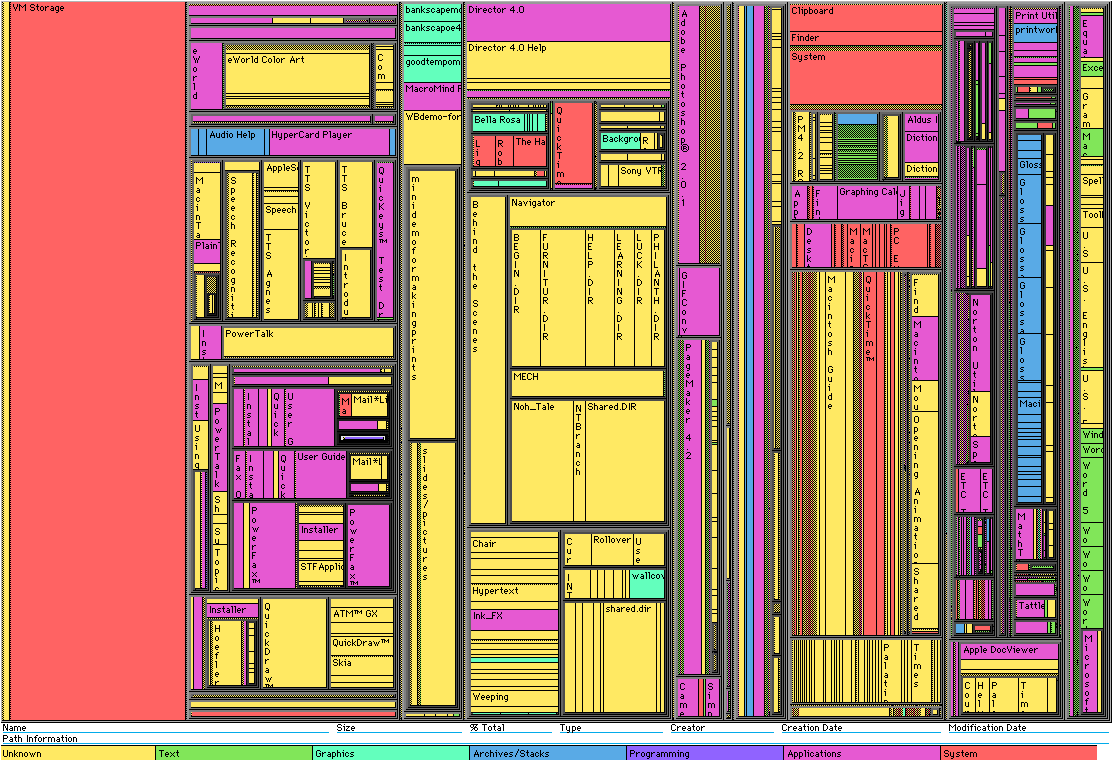
\includegraphics[width=.8\textwidth]{figures/intro/treemap_snd_colorful.png}
%     \caption{Earliest treemap method, Slice-and-Dice, displaying a file system.}
% \end{figure*}

\section{Visualizing temporal multidimensional data}
\label{sec:ch1_highdim}
%
Multidimensional (or high-dimensional) datasets have a number of observations (also called points or samples) where each observation has many attributes, also called variables, dimensions, or measurements. 
For datasets with relatively small numbers of observations and dimensions, techniques such as glyphs, parallel coordinate plots, table lenses, and scatterplot matrices can produce accurate and useful visual encodings.  
If a dataset has a large number of dimensions, roughly more than 4 to 5, however, multidimensional \emph{projections} tend to be the only scalable approach.  

Multidimensional projections take data in a high-dimensional space and project it into a lower-dimensional space, usually creating a 2D or 3D scatter plot, which we can directly visualize and reason about. In this transformation, the projection method attempts to create visual patterns that reflect the similarities or structure found in the high-dimensional space. That is, points which are similar -- according to any suitable similarity metric -- in the high-dimensional space are placed close in the 2D or 3D projection, and conversely.

Reflecting the similarities or structure found in the high-dimensional space can be interpreted in many ways, and the search for the ``best'' projection method has led to the proposal of a huge number of projection techniques.
There are many desirable traits projection methods can have, such as creating high distance or neighborhood preservation maps, scalability, simplicity, interpretability, out-of-sample capability, stability, and ease of use, among others. 
Optimizing a single one of these traits is already a challenging task that requires tradeoffs regarding the remaining traits. No single current method optimally satisfies all desirable requirements.

The trait that concerns us most in this thesis is \emph{stability}. Stability, or temporal coherence, needs to be taken into account when we project \emph{temporal} multidimensional data, that is, when the multidimensional data changes over time and, as illustrated in the previous section, we have multiple snapshots of the data. Most projection techniques are designed for static data. When used for time-dependent data, they usually fail to create a stable and suitable low dimensional representation. To follow the analogy with the dynamic treemaps discussed in Sec.~\ref{sec:ch1_tempo}: If we have a high-dimensional and temporal dataset, current projection methods usually create a visualization in which the observed points either do not change much while their corresponding high-dimensional counterparts change a lot; or they do change a lot whereas the high-dimensional data points only change little. Globally, the problem with projections is the same as that of treemaps -- they can produce false negatives and/or false positives which impair the ability of the user to judge about the data dynamics from seeing the visualization of the projected data.

\section{Temporal coherence}
\label{sec:ch1_coherence}
%
Treemaps and projections are incredibly useful techniques that, due to their compact and easy to interpret design, give unique insights into large and complicated datasets.
As mentioned so far, they were initially designed for static datasets. However, given the presence of dynamic datasets, the natural question arises on how to adapt them to handle such data, while avoiding the already discussed false-negative and false-positive problems. 

To illustrate the dynamic projections' instability, Fig.~\ref{fig:intro-pj-demo-instability} shows three different methods (G-PCA, TF-PCA, and TF-tSNE) projecting the same dataset, using a trail-like visual encoding. The \emph{gaussians} dataset is a 100-dimensional dataset of 2000 samples covering 10 distinct isotropic Gaussian distributions that collapse into 10 single points over 10 timesteps. Knowing the dataset, we can tell that G-PCA renders quite faithfully the data dynamics and structure; TF-PCA creates an artificial amount of spiraling; and TF-tSNE creates a very large amount of apparently random and unstable motion that is not present in the data.  For the purpose of the illustration in Fig.~\ref{fig:intro-pj-demo-instability}, detailed knowledge of the G-PCA, TF-PCA, and TF-tSNE projection methods is not needed. The point being made is that different projection methods show widely different visual insights in the \emph{same} dataset. As such, they clearly cannot be all right -- raising the question of which method is the best and, subsequently, how to define what a good method is in this context.

% https://docs.google.com/drawings/d/1XENnHkpmsl6AqJfx5l2b-H4bSuKonbjgjYY_E599Q5c/edit
\begin{figure*}[h]
    \centering
    \includegraphics[width=\linewidth]{figures/projection-algorithm/demo-instability-trails-rebuttal-with-color-3.eps}
   %  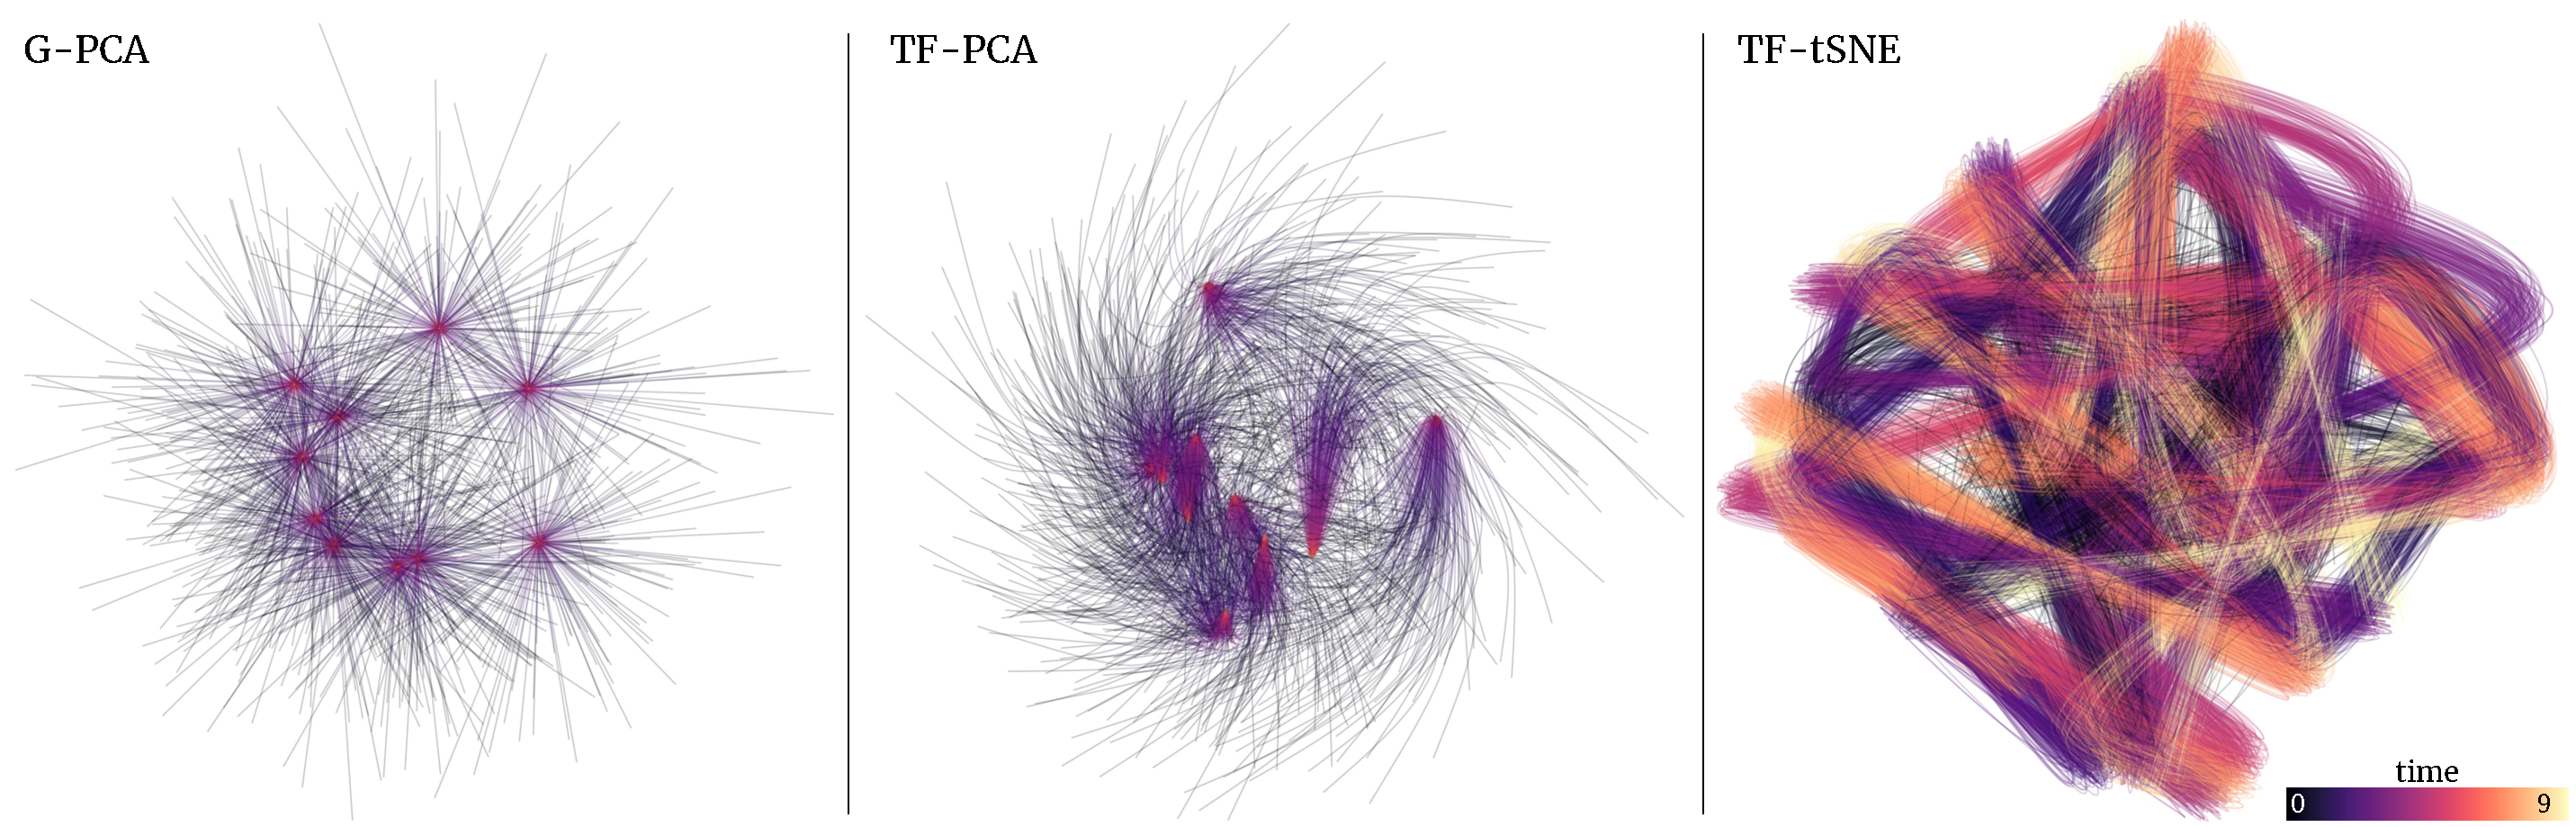
\includegraphics[width=0.48\linewidth]{figures/projection-algorithm/demo-instability-trails-rebuttal-with-color.pdf}
    \caption{A time-dependent collapsing 100-dimensional 10-Gaussian-distributions dataset (2000 points) is visualized by three projection methods. Point trails are colored by time (top) and class (bottom). The images show increasing amounts of instability artefacts.}
    \label{fig:intro-pj-demo-instability}
\end{figure*}

The same effect occurs when we create treemaps for time-dependent datasets. The top row of Fig.~\ref{fig:intro-tm-demo-instability} shows three snapshots/timesteps of the evolution of a simple weighted tree. The next two rows show two different treemapping algorithms creating rectangular treemap representations for the data (NMap and Squarified Treemap). Nmap creates a stable layout; that is, there are no significant changes in the positions of the cells driven by the small changes in the data, and the adjacencies in the layout remain the same over the evolution. In contrast, in the Squarified Treemap layout, cell \emph{d} (red) keeps changing its relative position. When dealing with more complicated datasets, this movement can happen for multiple cells simultaneously, making it impossible to accurately reason about the data and the change in the data. As for the projection example in Fig.~\ref{fig:intro-pj-demo-instability}, the issue is not understanding how NMap or Squarified Treemap work. Rather, the higher level question is that (at least) one of these methods is suboptimal, and, as a consequence, how to measure the quality of a dynamic treemapping method.

\begin{figure*}[h]
    \centering
    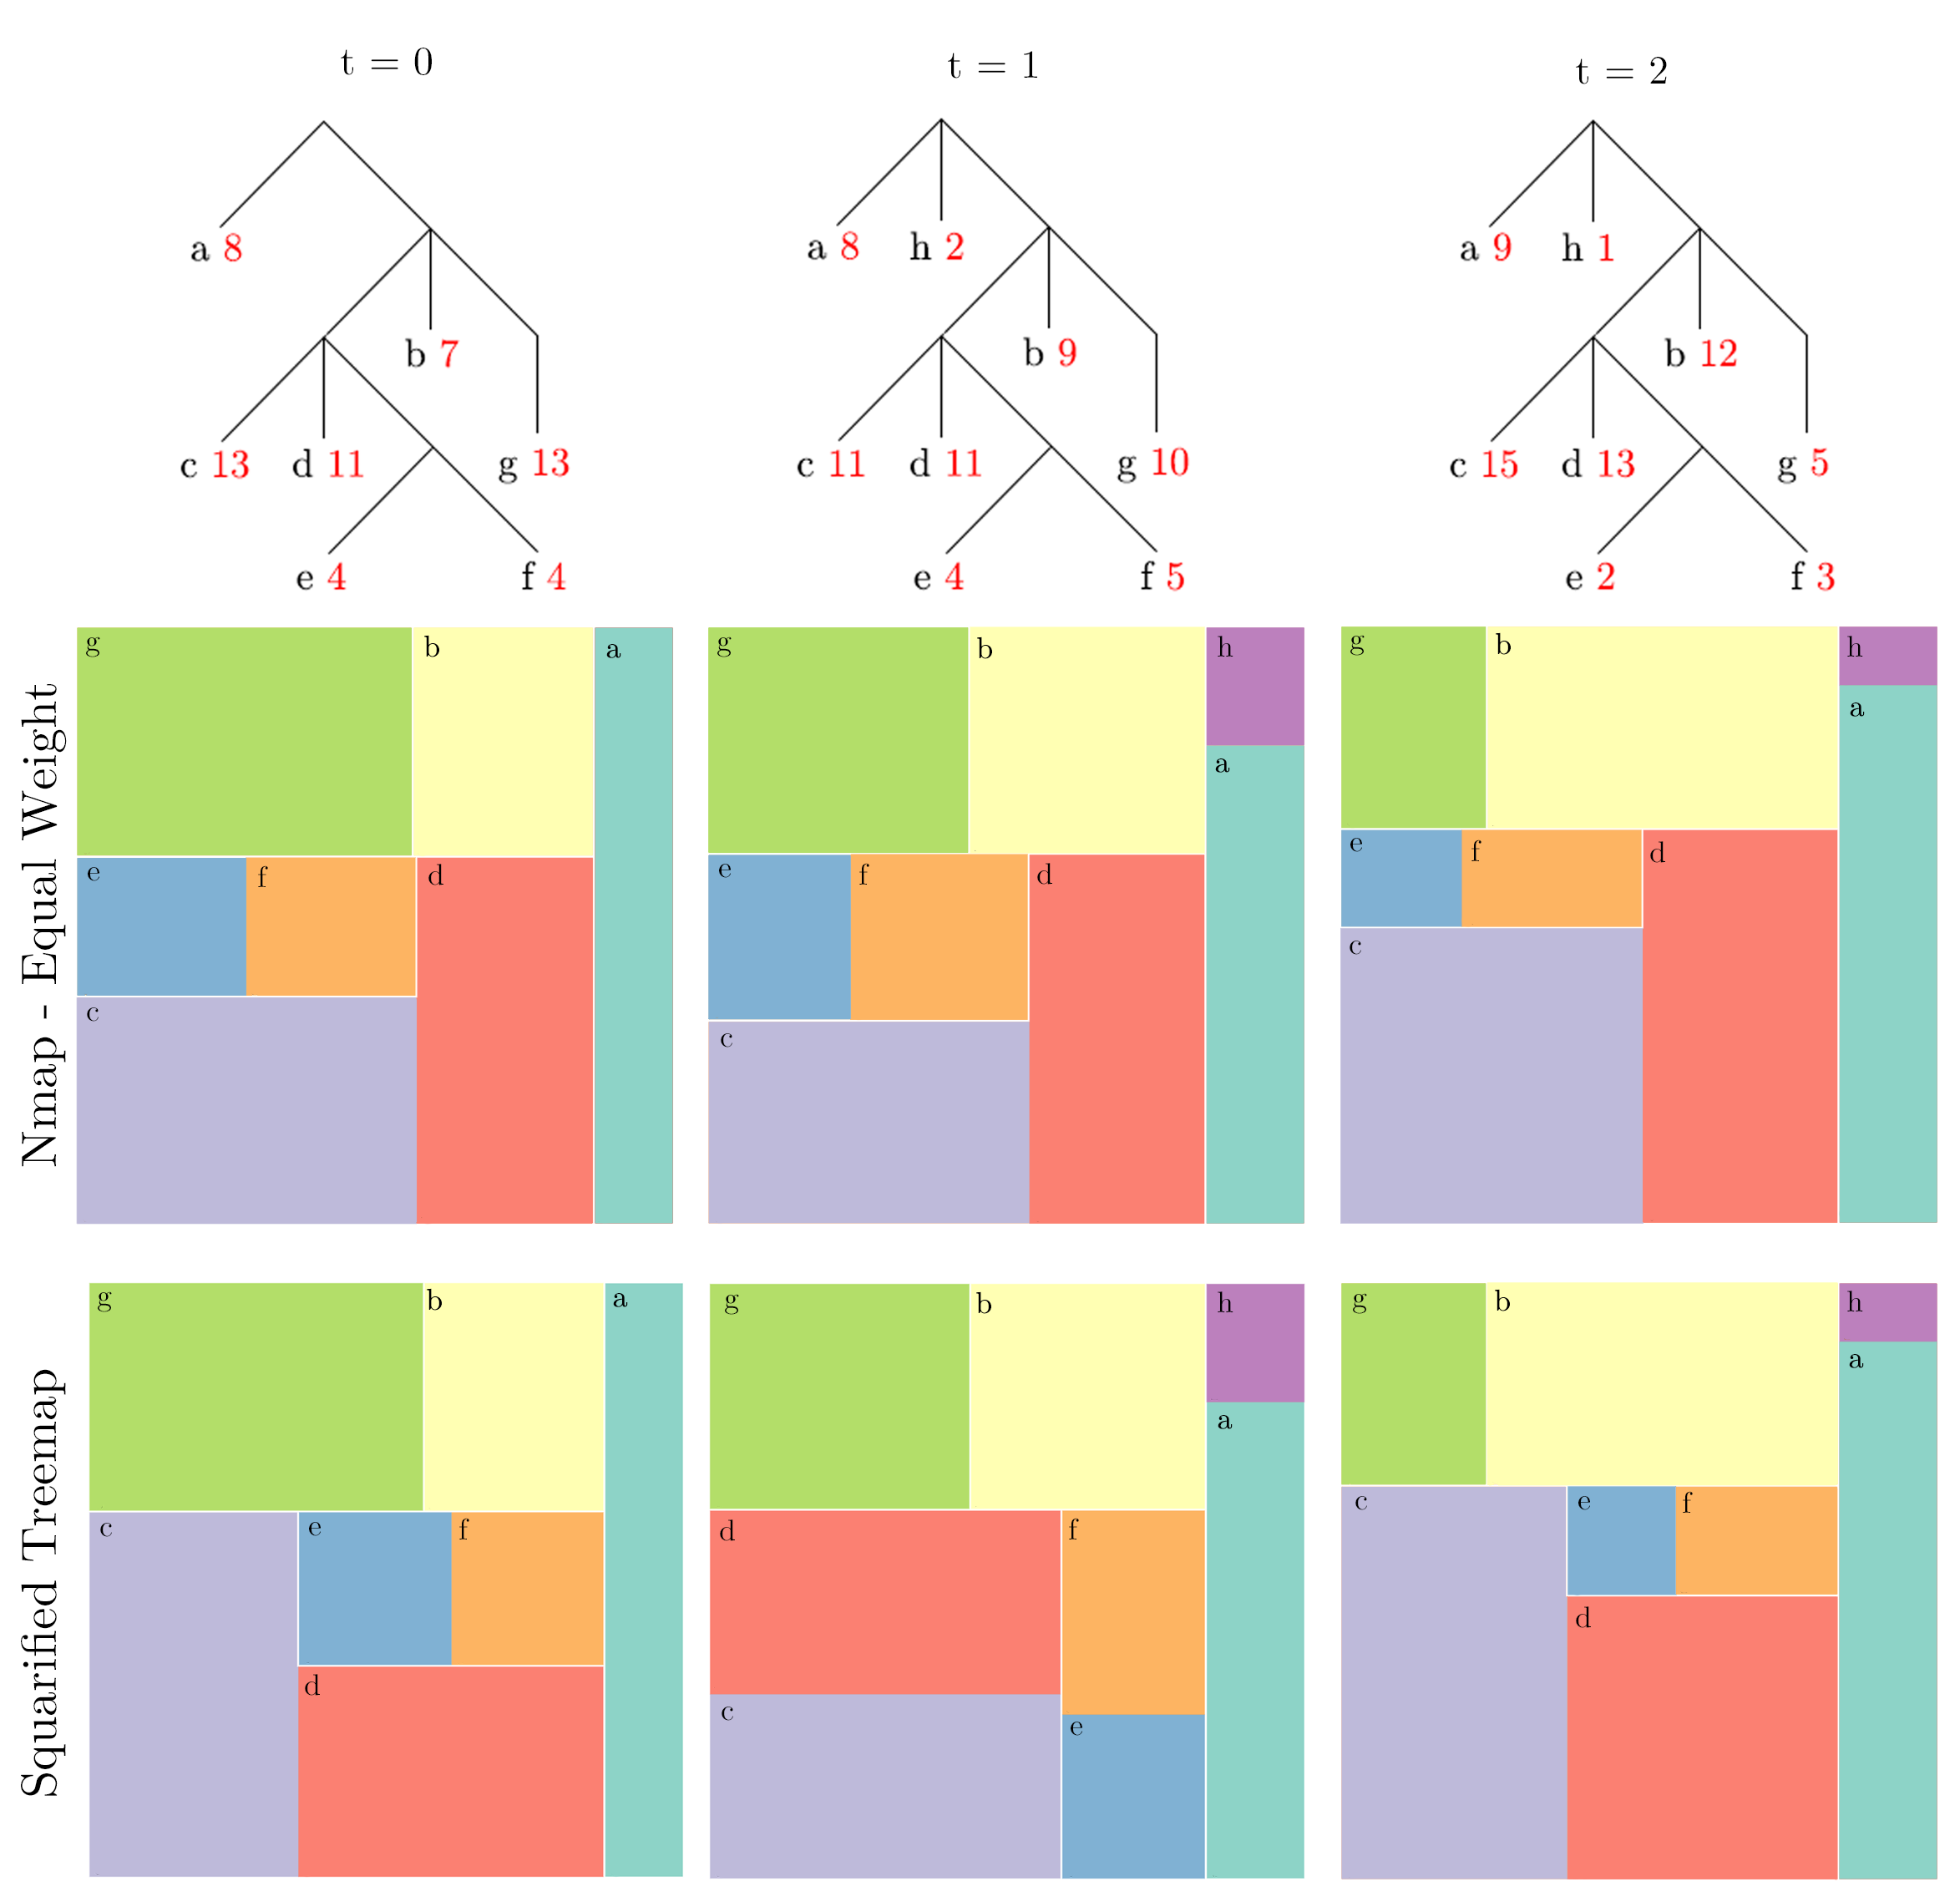
\includegraphics[width=\linewidth]{figures/intro/mov_sub_new.png}
    \caption{Layouts generated by NMap\,\cite{xxx} and Squarified Treemap\,\cite{xxx} for a sample hierarchical dataset
    of 3 time steps. We see how NMap is more stable, and similar in aspect ratio, than Squarified Treemap.}
    \label{fig:intro-tm-demo-instability}
\end{figure*}

To create faithful and useful representation of temporal data, we need to be able to ensure \emph{temporal coherence}: Small changes in the data should result in small changes in the visualization; large changes in the data should result in large changes in the visualization. All other mappings of changes in the data to changes in the visualization are arguably bad. Simply put, we want to guarantee that changes perceived by the viewer are due to changes in the data alone. However, while this 
desiderate is -- we argue -- clear and evident, there are no treemapping or projection algorithms that comply with it. Even more fundamentally, the very issue of relating data change to visualization change in these two contexts, and deciding what is a `good' mapping of the former to the latter, is not defined by theory or metrics to gauge it.

\section{Objectives and contributions}

We have argued that treemaps and projections are valuable tools for making sense of hierarchical and multidimensional data, respectively. However, when it comes to applying these visual encodings to \emph{time-dependent} data, these methods tend to show undesirable traits; and only limited research effort has been dedicated to understanding, testing, and developing methods that preserve temporal coherence. This research gap leads us to this thesis' high-level research question, stated next as

\subsection*{How to extend projections and treemaps to stably, accurately, and scalably handle temporal multivariate and hierarchical data?}

To address this question, there are three components that must be satisfied in either track. We must be able to

\subsection*{A. Develop ways of accurately measuring stability}

To evaluate the stability of a dynamic treemap or dynamic projection, we need to have reliable measurement tools that quantify the relationship between data change and visual change.

For treemaps, we developed the \emph{Unavoidable Change} metric, based on the mathematically proven minimum change that cells would need to undergo to accommodate the data change, and \emph{Baseline Treemaps}, a similar method to approximate the minimum amount of change that any time-dependent treemap must incur when data changes. We also proposed a set of stability metrics for dynamic projections based on the mathematics of visual quality metrics.
Before our work, there were no methods designed to measure instability that took into consideration data change -- they only looked at visual change, which can be deceiving. As such, we argue that our work provides a contribution to the fundamentals of using treemaps for reliably depicting dynamic hierarchical data.

\subsection*{B. Evaluate methods in the literature considering the tradeoff between stability and visual quality}

As already hinted, tens of methods for constructing treemaps and projections exist. However, and as also already hinted, few if none of these methods were gauged from the perspective of stability -- one reason thereof being the lack of a \emph{measure} for stability. Having developed such a measure, as mentioned above at point (A), we next use it to produce comprehensive evaluations for dynamic treemaps and projections from the stability perspective. Our contributions in this direction entail work along the following axes:

\begin{itemize}
    \item \emph{Metrics:} We proposed and implemented a novel set of metrics that reliably measures visual quality and stability.
    \item \emph{Datasets:} Since there was no previous extensive evaluation or benchmark designed for testing dynamic treemaps or projections, we collected and/or generated a comprehensive collection of datasets that drove our evaluations. 
    \item \emph{Methods:} Collection, implementation, and proposal of several dynamic treemap and projection algorithms. Most of the work on the topic up until our work was conjectural and not quantitatively tested.  Simply put, there was no central collection of algorithms that one could use to compare and gauge the performance of dynamic treemaps and dynamic projections. We claim that work solved a large part of this challenge.
    \item \emph{Analysis:} We combined the previous axes into comprehensive insights into dynamic projections and treemaps. Simply put, we generated quantitative and qualitative evidence showing how existing dynamic projection and treemap algorithms compare to each other, allowing both researchers and practitioners to choose which subset of algorithms are best suited to extend next, respectively directly use in practice.
\end{itemize}

\subsection*{C. Design state-of-the-art methods that strike a good balance between stability and visual quality}

Once the tools necessary to test and compare dynamic treemaps and projections were in place, we were able to leverage the gained insights to produce state-of-the-art algorithms that strike a better balance between stability and visual quality.

Specifically, we have developed Greedy Insertion Treemap (GIT), a stable and scalable state-aware method for displaying dynamic treemaps. Compared to all treemapping algorithms that we were aware of at the time of GIT's development, we showed that GIT provides a better tradeoff between spatial quality and stability, therefore surpassing its competitors. Moreover, GIT is simple to implement, generic, and computationally scalable.

Regarding projections, we proposed PCD-tSNE and LD-tSNE, two neighborhood-based projection methods that use global guides to steer the projected points. This avoids unstable movement that does not encode data dynamics while keeping, at the same time, the highly praised visual quality of the t-Stochastic Neighborhood Embedding (t-SNE) projection method\,\cite{xxx}, arguably the best known high-quality projection method used nowadays for high-dimensional data. As for GIT, PCD-tSNE and LD-tSNE are generic methods, with good computational scalability.

\bigbreak

Lastly, it is important to mention that all aspects of our research are open. All the code and data is organized and available online to facilitate further research on dynamic treemaps and projections. This directly supports our answering of the earlier mentioned research questions -- which, besides theory, require materials such as data and software for interested researchers and practitioners to replicate, extend, and ultimately use our contributions.

\section{Organization of the thesis}

\alex{Here and later: I added \cite{xxx} reference placeholders for the obvious things - like the 1st time you refer to a term or method. Please fill these in. It's trivial to do so. Will add more as I read/correct more Please pedantically fill these in!}

\eduardo{will add refs later}

\alex{Yes please do. Also, in sec 1.5, be short: simply list the chapters and say what you do in which and how that relates to what PREVIOUS sections in this chapter mention. Easy. Just, like, 1..2 paragraphs per chapter, not more.}

\eduardo{(explanation for unavoidable change metric is not in the text yet -- software visualization paper)}

\eduardo{quotes come from here http://www.cs.umd.edu/hcil/treemap-history/index.shtml}

